\chapter{Java 数组和字符串}
\label{chp:Java-array-and-string}

\section*{基本信息}
\sline
\begin{description}
\item[课程名称:] Java应用与开发
\item[授课教师:] 王晓东
\item[授课时间:] 第二周
\item[参考教材:] 本课程参考教材及资料如下:
  \begin{itemize}
  \item 陈国君主编,Java程序设计基础(第5版),清华大学出版社,2015.5
  \item Bruce Eckel, Thinking in Java (3rd)
  \end{itemize}
\end{description}

\section*{教学目标}

\sline

\begin{enumerate}
\item 掌握Java数组的概念
\item 学会一维数组和二维数组的使用;认识Arrays类,掌握操作数组相关方法
\item 掌握Java字符串的概念,字符串与数组的关系;学会String类常用字符串操作方法
\end{enumerate}

\section*{授课方式}

\sline
\begin{description}
\item[理论课:] 多媒体教学、程序演示
\item[实验课:] 上机编程
\end{description}

\newpage
\section*{教学内容}
\sline

\section{数组的概念}

数组是相同数据类型的元素按一定顺序排列的集合。在Java语言中,数组元素既可以为基本数据类型,也可以为对象。

\kgtip{Java的内存分配(基础)}

\begin{description}
\item [栈内存] 存放定义的基本类型的变量和对象的引用变量,超出作用域将自动释放。
\item [堆内存] 存放由new运算符创建的对象和数组,由Java虚拟机的自动垃圾回收器来管理。
\end{description}

Java数组的主要特点包括以下方面:

\begin{itemize}
\item 数组是相同数据类型的元素的集合;
\item 数组中的各元素有先后顺序,它们在内存中按照这个先后顺序连续存放;
\item 数组的元素用整个数组的名字和它自己在数组中的顺序位置来表示。
\end{itemize}

{\Blue\kai 例如,a[0]表示名字为a的数组中的第一个元素,a[1]表示数组a的第二个元素,依次类推。}

\section{一维数组}

\subsection{创建数组}

创建Java数组一般需经过三个步骤:

\begin{enumerate}
\item 声明数组;
\item 创建内存空间;
\item 创建数组元素并赋值。
\end{enumerate}

\samplecode{一维数组创建声明和内存分配}

\begin{javaCode}
  int[] x;  //声明名称为x的int型数组,未分配内存给数组
  x = new int[10];   //x中包含有10个元素,并分配空间
\end{javaCode}

\begin{javaCode}
  int[] x = new int[10];   //声明数组并动态分配内存
\end{javaCode}

\descript{说明}

用new分配内存的同时,数组的每个元素都会自动赋默认值,整型为0,实数为0.0,布尔型为false,引用型为null。

\subsection{一维数组的初始化}

若在声明数组时进行赋值即初始化,称为静态内存分配。

\begin{javaCode}
  数据类型[] 数组名 = {初值0,初值1,…,初值n};
\end{javaCode}

\samplecode{一维数组静态初始化}

\begin{javaCode}
  int[] a = {1,2,3,4,5};
\end{javaCode}

\descript{注意}

在Java程序中声明数组时,无论用何种方式定义数组,都不能指定其长度。

\section{二维数组}

Java中无真正的多维数组,只是数组的数组。

\subsection{二维数组的声明和内存分配}

\begin{javaCode}
  数据类型[][] 数组名;
  数组名 = new 数据类型 [行数][列数];
  数据类型[][] 数组名 = new 数据类型 [行数][列数];
\end{javaCode}

\begin{figure}[htb]
\centering
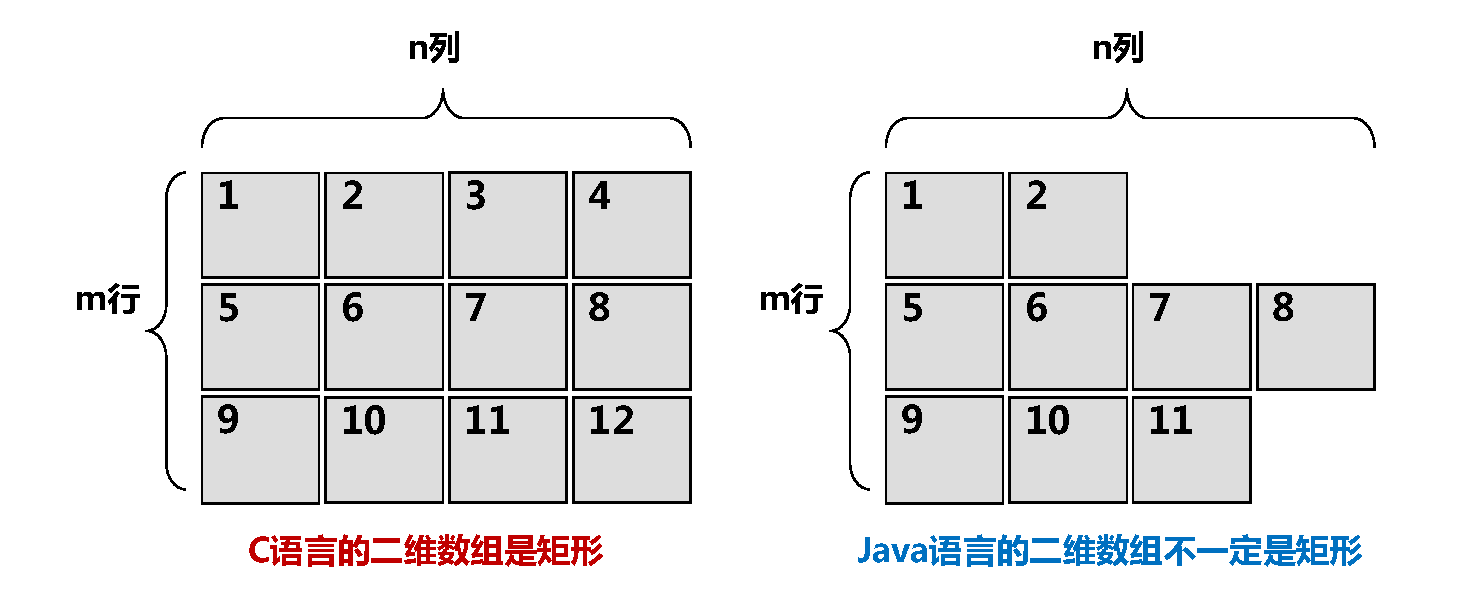
\includegraphics[width=\textwidth]{images/Java-array-and-string/fig-2-dim-array.pdf}
\caption{Java和C语言数数组}
\label{fig:java-and-c-array}
\end{figure}

\subsection{二维数组定义的含义}

\begin{itemize}
\item Java中的二维数组看作是由多个一维数组构成
\item 二维数组申请内存必须指定{\Red 高层维数}\\
  \fbox{int[][] myArray1 = new int[10][];}\\
  \fbox{int[][] myArray2 = new int[10][3];}
\item \fbox{int[][] x;}\\
  {\kai\Blue 表示定义了一个数组引用变量x,第一个元素为x[0],最后一个为x[n-1],其长度不确定}
\item \fbox{x = new int[3][];}\\
  {\kai\Blue 表示数组x有三个元素,每个元素都是int[]类型的一维数组,分别为int x[0][]、int[] x[1]、int[] x[2]}\\
  \fbox{x[0] = new int[3];  x[1] = new int[2];}\\
  {\kai\Blue 给x[0]、x[1]、x[2]赋值(长度可以不一样)}
\end{itemize}

\subsection{二维数组赋初值}

\begin{javaCode}
  int[][] a = {{11,22,33,44}, {66,77,88,99}};
\end{javaCode}

\descript{注意}

声明多维数组并初始化时不能指定其长度,否则出错。



\section{Arrays类}

java.util.Arrays工具类能方便地操作数组,它提供的所有方法都是静态的。该类具有以下功能:

\begin{description}
\item[给数组赋值] 通过fill方法。
\item[对数组排序] 通过sort方法。
\item[比较数组] 通过equals方法比较数组中元素值是否相等。
\item[查找数组元素] 通过binarySearch方法能对排序好的数组进行二分查找法操作。
\item[复制数组] 把数组复制成一个长度为length的新数组。
\end{description}

\samplecode{Array操作示例}

\begin{javaCode}
  /*
  * 数组比较 equals
  */
  String[] str1 = { "1", "2", "3" };
  String[] str2 = { "1", "2", new String("3") };
  System.out.println(Arrays.equals(str1, str2)); // 结果是true

  /*
  * 数组排序 sort
  */
  int[] score = { 79, 65, 93, 64, 88 };

  // 将数组转换为字符串
  String str = Arrays.toString(score);
  System.out.println("原数组为:" + str);

  Arrays.sort(score); // 作用是把一个数组按照有小到大进行排序,会改变原score而不是创建新对象

  // 将数组转换为字符串
  System.out.println("排序后数组为:" + Arrays.toString(score));

  /*
  * 把数组中的所有元素替换成一个值 fill
  */
  int[] num = { 1, 2, 3 };
  Arrays.fill(num, 6); // 参数1:数组对象;参数2:替换的值
  System.out.println(Arrays.toString(num)); // 打印结果:[6, 6, 6]

  /*
  * 通过二分法查询元素值在数组中的下标 binarySearch
  */
  char[] a = { 'a', 'b', 'c', 'd', 'e' };
  int i = Arrays.binarySearch(a, 'd');
  System.out.println(i); // 结果是:3

  char[] b = { 'e', 'a', 'c', 'b', 'd' };
  Arrays.sort(b);
  int j = Arrays.binarySearch(b, 'e');
  System.out.println(j); // 结果是:4

  /*
  * 把数组内容复制到一个新数组中 copyOf
  */
  int[] c = { 1, 2, 3 };
  int[] d = Arrays.copyOf(c, c.length + 2); // 参数1:原数组 参数2:新数组的长度
  System.out.println("原数组为:" + Arrays.toString(c));
  System.out.println("复制后的新数组为:" + Arrays.toString(d));  
\end{javaCode}


\section{字符串}

字符串是用一对双引号括起来的字符序列。Java语言中,字符串常量或变量均用类实现。

\subsection{字符串变量的创建}

\samplecode{格式1}

\begin{javaCode}
  String s;                  //声明字符串型引用变量s,此时s的值为null
  s = new String("Hello");   //在堆内存中分配空间,并将s指向该字符串首地址
\end{javaCode}

\samplecode{格式2}

\begin{javaCode}
  String s = new String("Hello");
\end{javaCode}

\samplecode{格式3}

\begin{javaCode}
  String s = "Hello";
\end{javaCode}

\subsection{String类的常用方法}

\samplecode{求字符串长度}

\begin{javaCode}
  String str = new String("asdfzxc");
  int strlength = str.length(); //strlength = 7
\end{javaCode}

\samplecode{获取字符串某一位置字符}

\begin{javaCode}
  char ch = str.charAt(4); //ch = z
\end{javaCode}

\samplecode{提取子串}

\begin{javaCode}
  String str2 = str1.substring(2); //str2 = "dfzxc"
  String str3 = str1.substring(2,5); //str3 = "dfz"
\end{javaCode}

\samplecode{字符串连接}

\begin{javaCode}
  String str = "aa".concat("bb").concat("cc");
  String str = "aa" + "bb" + "cc"; // 相当于上一行
\end{javaCode}


\samplecode{字符串比较}

\begin{javaCode}
  String str1 = new String("abc");
  String str2 = new String("ABC");
  int a = str1.compareTo(str2);  //a>0
  int b = str1.compareTo(str2);  //b=0
  boolean c = str1.equals(str2); //c=false
  boolean d = str1.equalsIgnoreCase(str2); //d=true
\end{javaCode}

\samplecode{字符串中字符的大小写转换}

\begin{javaCode}
  String str = new String("asDF");
  String str1 = str.toLowerCase(); //str1 = "asdf"
  String str2 = str.toUpperCase(); //str2 = "ASDF"
\end{javaCode}

\samplecode{字符串中字符的替换}

\begin{javaCode}
  String str = "asdzxcasd";
  String str1 = str.replace('a','g'); //str1 = "gsdzxcgsd"
  String str2 = str.replace("asd","fgh"); //str2 = "fghzxcfgh"
  String str3 = str.replaceFirst("asd","fgh"); //str3 = "fghzxcasd"
  String str4 = str.replaceAll("asd","fgh"); //str4 = "fghzxcfgh"
\end{javaCode}

\subsection{理解Java字符串}

\samplecode{String.java部分代码}

\begin{javaCode}
  public final class String
  implements java.io.Serializable, Comparable<String>, CharSequence { //1

    /** The value is used for character storage. */
    private final char value[]; //2
    
    /** The offset is the first index of the storage that is used. */
    private final int offset;
    
    /** The count is the number of characters in the String. */
    private final int count;
    
    /** Cache the hash code for the string */
    private int hash; // Default to 0

    /** use serialVersionUID from JDK 1.0.2 for interoperability */
    private static final long serialVersionUID = -6849794470754667710L;
    ........

    public String substring(int beginIndex, int endIndex) { //3
      if (beginIndex < 0) {
        throw new StringIndexOutOfBoundsException(beginIndex);
      }
      if (endIndex > count) {
        throw new StringIndexOutOfBoundsException(endIndex);
      }
      if (beginIndex > endIndex) {
        throw new StringIndexOutOfBoundsException(endIndex - beginIndex);
      }
      return ((beginIndex == 0) && (endIndex == count)) ? this :
      new String(offset + beginIndex, endIndex - beginIndex, value);
    }
}
\end{javaCode}

\begin{enumerate}
\item String类是final类,即意味着String类不能被继承,并且它的成员方法都默认为final方法。
\item 从String类的成员属性可以看出String类其实是通过char数组来保存字符串的。
\item 无论是substring还是concat操作等都不是在原有的字符串上进行的,而是重新生成了一个新的字符串对象,最原始的字符串并没有被改变。

\end{enumerate}

\descript{说明}

String对象一旦被创建就是固定不变的,对String对象的任何操作都不影响到原对象,而是会生成新的对象。